\documentclass[xcolor=dvipsnames
              %,handout
              ]{beamer} 

\usetheme{Madrid} 
%\setbeamertemplate{blocks}[shadow=false] 
\setbeamertemplate{navigation symbols}{} 
\setbeamertemplate{items}[square]
\setbeamertemplate{sections/subsections in toc}[square]

\definecolor{myblueend}{rgb}{0.058,0.132,0.42}
\definecolor{mybluemiddle}{rgb}{0.31,0.45,0.64}
\definecolor{mybluestart}{rgb}{0.17,0.28,0.48}
\definecolor{mygreen}{rgb}{0,0.7,0}
\definecolor{mylightgreen}{rgb}{0.7,1,0.7}
\definecolor{mylightblue}{rgb}{0.7,0.7,1}
\definecolor{mylightblack}{rgb}{0.7,0.7,0.7}
\definecolor{mylightred}{rgb}{1,0.7,0.7}
\definecolor{oproverblue}{RGB}{12,83,144}
\definecolor{oproveryellow}{RGB}{255,156,55}
\definecolor{mydarkgreen}{rgb}{0.17,0.48,0.28}
\definecolor{mydarkred}{rgb}{0.48,0.28,0.17}
\definecolor{grey}{rgb}{0.7,0.7,0.7}

%\setbeamercolor{palette primary}{fg=white,bg=mybluestart}
%\setbeamercolor{palette secondary}{fg=white,bg=mybluestart}
%\setbeamercolor{palette tertiary}{fg=white,bg=mybluestart}
%\setbeamercolor{palette quaternary}{fg=white,bg=mybluestart}
\setbeamercolor{palette primary}{fg=white,bg=oproverblue}
\setbeamercolor{palette secondary}{fg=white,bg=oproverblue}
\setbeamercolor{palette tertiary}{fg=white,bg=oproverblue}
\setbeamercolor{palette quaternary}{fg=white,bg=oproverblue}
\setbeamercolor{titlelike}{parent=palette quaternary}

\setbeamercolor{item}{fg=oproverblue}
\setbeamercolor{block title}{fg=white,bg=oproverblue}
\setbeamercolor{block title example}{fg=white,bg=oproveryellow}
%\setbeamercolor{block title alert}{fg=white,bg=mydarkred}

\usefonttheme{serif}

%%
%% TOOLS
%% 
\newcommand{\opensmt}{{\sc OpenSMT}\xspace}
\newcommand{\yices}{{\sc Yices}\xspace}
\newcommand{\mathsat}{{\sc MathSAT}\xspace}
\newcommand{\cvcfour}{{\sc CVC4}\xspace}
\newcommand{\zthree}{{\sc Z3}\xspace}
\newcommand{\boolector}{{\sc Boolector}\xspace}
\newcommand{\verit}{{\sc veriT}\xspace}
\newcommand{\stp}{{\sc STP}\xspace}
\newcommand{\minisat}{{\sc MiniSAT}\xspace}
%%
%% BOOLEAN OPERATORS
%%
\newcommand{\swedge}{\,\wedge\,}
\newcommand{\svee}{\,\vee\,}
\newcommand{\impl}{\,\rightarrow\,}
%%
%% SMTLIB LOGICS
%% 
\newcommand{\Idl}{\ensuremath{\mathcal{IDL}}\xspace}
\newcommand{\Rdl}{\ensuremath{\mathcal{RDL}}\xspace}
\newcommand{\Uf}{\ensuremath{\mathcal{UF}}\xspace}
\newcommand{\Lia}{\ensuremath{\mathcal{LIA}}\xspace}
\newcommand{\Lra}{\ensuremath{\mathcal{LRA}}\xspace}
\newcommand{\Arrays}{\ensuremath{\mathcal{A}}\xspace}
\newcommand{\Bitvectors}{\ensuremath{\mathcal{BV}}\xspace}
\newcommand{\T}{\ensuremath{\mathcal{T}}\xspace}
\newcommand{\B}{\ensuremath{\mathcal{B}}\xspace}
%%
%% SETS
%%
\newcommand{\Int}{\ensuremath{\mathbb{Z}}\xspace}
\newcommand{\Rat}{\ensuremath{\mathbb{Q}}\xspace}
\newcommand{\Rea}{\ensuremath{\mathbb{R}}\xspace}
\newcommand{\Boo}{\ensuremath{\mathbb{B}}\xspace}
%%
%% SORTS
%%
\newcommand{\SInt}{{\tt Int}\xspace}
\newcommand{\SRea}{{\tt Real}\xspace}
\newcommand{\SBoo}{{\tt Bool}\xspace}
\newcommand{\SBv}[1]{{\tt BV}$_{[#1]}$\xspace}
%%
%% SMT specific
%%
\newcommand{\tconflict}{\T-conflict\xspace}
\newcommand{\tconflicts}{\T-conflicts\xspace}
\newcommand{\tterm}{\T-term\xspace}
\newcommand{\tterms}{\T-terms\xspace}
\newcommand{\tatom}{\T-atom\xspace}
\newcommand{\tatoms}{\T-atoms\xspace}
\newcommand{\tlit}{\T-literal\xspace}
\newcommand{\tlits}{\T-literals\xspace}
\newcommand{\tformula}{\T-formula\xspace}
\newcommand{\batom}{\B-atom\xspace}
\newcommand{\batoms}{\B-atoms\xspace}
\newcommand{\blit}{\B-literal\xspace}
\newcommand{\blits}{\B-literals\xspace}
\newcommand{\babst}[1]{#1^{\B}}
\newcommand{\tsolver}{\T-solver\xspace}
\newcommand{\tsolvers}{\T-solvers\xspace}
%%
%% SAT specific
%%
\newcommand{\dec}[2]{\stackrel{\textcolor{oproveryellow}{#2}}{#1}}
%%
%% BIT-VECTORS
%%
\newcommand{\w}[2]{\ensuremath{#1_{[#2]}}}
\newcommand{\band}{\,{\bf AND}\,}
\newcommand{\bor}{\,{\bf OR}\,}
\newcommand{\bnot}{{\bf NOT}\,}
\newcommand{\bitandsymb}{\,\, {\bf AND}}
\newcommand{\bit}[2]{#1\ensuremath{^#2}}
%%
%% IDL graphs
%%
\newcommand{\idlnode}[2]{\frac{#1}{#2}}
%%
%% LRA Solver
%%
\newcommand{\bas}{\ensuremath{\mathcal{B}}\xspace}
\newcommand{\nonbas}{\ensuremath{\mathcal{N}}\xspace}
%%
%% EUF graphs
%%
%\newcommand{\nod}[3]{\frac{{#1}}{#2,#3}}
\newcommand{\nod}[3]{
  \tiny
  \begin{array}{c}
    #1 \\
    #2, #3
  \end{array}
}
%%
%% MISC
%%
\newcommand{\Lbrack}{\ensuremath{[\mspace{-3mu}[}}
\newcommand{\Rbrack}{\ensuremath{]\mspace{-3mu}]}}
\newcommand{\inter}[1]{\ensuremath{\Lbrack #1 \Rbrack}}
\newcommand{\COMMENT}[1]{}
\newcommand{\hl}[1]{\colorbox{oproveryellow}{\bf #1}}
\newcommand{\colfou}[1]{\textcolor{grey}{#1}}
\newcommand{\formulae}{formul\ae\xspace}
\newcommand{\smtsolvers}{SMT-solvers\xspace}
\newcommand{\smtsolver}{SMT-solver\xspace}
\newcommand{\satsolvers}{SAT-solvers\xspace}
\newcommand{\satsolver}{SAT-solver\xspace}
\newcommand{\bitvectors}{Bit-Vectors\xspace}
\newcommand{\bitvector}{Bit-Vector\xspace}
\newcommand{\colone}[1]{\textcolor{red}{#1}}
\newcommand{\coltwo}[1]{\textcolor{mygreen}{#1}}
\newcommand{\coloneat}[2]{\textcolor<#2>{red}{#1}}
\newcommand{\coltwoat}[2]{\textcolor<#2>{mygreen}{#1}}
\newcommand{\colfouat}[2]{\textcolor<#2>{grey}{#1}}
\newcommand{\claset}{\mathcal{C}}
\newcommand{\ra}[1]{\renewcommand{\arraystretch}{#1}}

\usepackage{epsfig}
\usepackage{graphicx}
\usepackage{color}
\usepackage{amstext}
\usepackage{amssymb}
\usepackage{amsfonts}
\usepackage{amsmath}
\usepackage{amsthm}
\usepackage{xspace}
\usepackage{multirow}
\usepackage{tabularx,colortbl}
\usepackage{alltt}
\usepackage{bussproofs}
\usepackage{algorithm2e}
\usepackage{datetime}


\title[Intro to MC]{Satisfiability Modulo Theories\\ Lecture 8 - Introduction to SMT-based Model-Checking \\ {\tiny (slides revision: \today, \currenttime)}}
\author[R. Bruttomesso]{\large Roberto Bruttomesso}
\date{15 Dicembre 2011}
\institute[SMT]{\large Seminario di Logica Matematica \\ (Corso Prof. Silvio Ghilardi)}
\logo{ \vspace{-6pt} 
\includegraphics[scale=0.15]{imgs/logo-ita.png} }

\begin{document}

\frame{\titlepage}

\begin{frame}
  \frametitle{Outline}
  \tableofcontents
\end{frame}

\section{Basics}
\begin{frame}
  \frametitle{Introduction}

  Model-Checking is a set of techniques to approach the verification
  of a system (e.g., a hardware circuit, a program, a protocol)
  \vfill
  It was proposed by Clarke-Emerson and Sifakis-Quine
  as a way of automatically prove properties of a system
  \vfill
  The authors received the Turing Award in 2007
  \vfill
  The idea of model-checking was in 
  contrast with the established ``philosophy'' at that time ($\sim$ 1980) 
  which was suggesting semi-automatic human-driven approaches: 
  MC is loved by industry because of this ``push-button'' characteristic

\end{frame}

\subsection{Modeling}

\begin{frame}
  \frametitle{Model-Checking - Modeling}

  In MC we model the behavior of a system with the
  notion of {\bf state}. A state is a configuration of
  the system at a particular time instant 
  \vfill
  The system can change state by means of a {\bf transition}
  \vfill
  We are interested in a {\bf property} of the system
  \vfill
  \pause
  Example:
  \begin{itemize}
    \item System: a washing machine
    \item A state: ``the door is open and the engine is off''
    \item A transition: ``if the door is open then close the door''
    \item A property: ``When the engine is on, the door is closed''
  \end{itemize}

\end{frame}

\begin{frame}
  \frametitle{System to Model}

  \begin{center}
  
\includegraphics[scale=.67]{imgs/cheap-washing-machine-edit.png}
  \end{center}

\end{frame}

\begin{frame}
  \frametitle{Modeling - States}

  State variables can be used to describe a particular state
  \vfill
  \begin{center}
  \begin{tabular}{ll}
    \hline
    State variable & Values \\
    \hline
    door           & open, closed \\
    tray           & empty, filled \\ 
    engine         & off, on \\
    \hline
  \end{tabular}
  \end{center}
  \vfill\pause
  E.g.:
  \begin{center}
  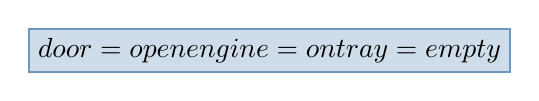
\begin{tikzpicture}[auto]

%
% Styles
%
\tikzstyle{vertex} = [rectangle,draw=oproverblue!60,fill=oproverblue!20,thick]

\node[vertex] (x) at ( 0, 0)  {$\nodd{door=open}{engine=on}{tray=empty}$};

\end{tikzpicture}

  \end{center}
  which stands for ``the door is open, the engine is on, and the tray is empty''.\pause
  How many different states can we describe with our state variables ? 

\end{frame}

\begin{frame}
  \frametitle{Modeling - States}

  \begin{center}
  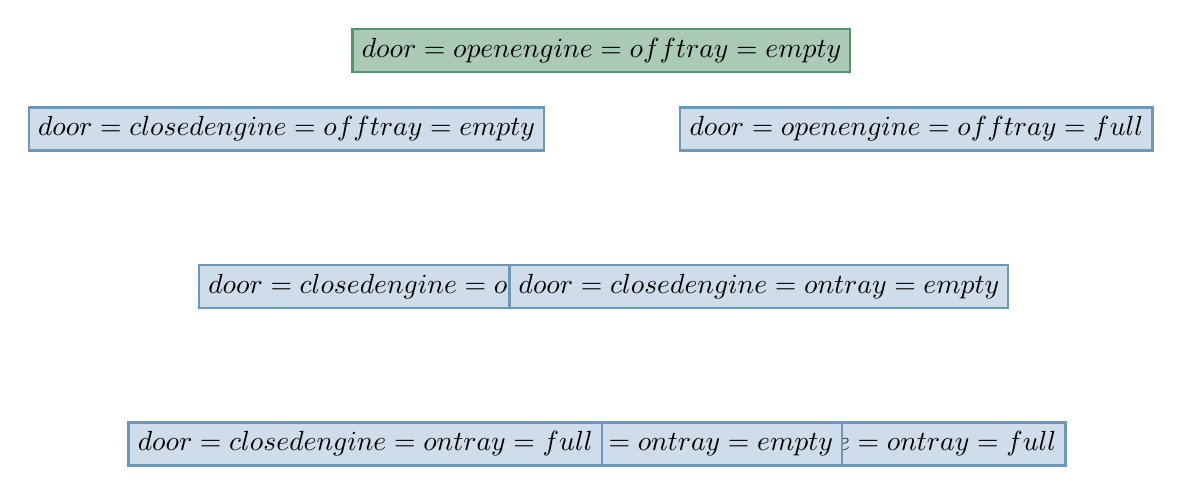
\begin{tikzpicture}[auto]

%
% Styles
%
\tikzstyle{state} = [rectangle,draw=oproverblue!60,fill=oproverblue!20,thick]
\tikzstyle{initialstate} = [rectangle,draw=mydarkgreen!80,fill=mydarkgreen!40,thick]

\node[initialstate] (000) at (  0,  -1)  {$\nodd{door=open}{engine=off}{tray=empty}$};
\node[state] (100) at ( -4, -2)  {$\nodd{door=closed}{engine=off}{tray=empty}$};
\node[state] (001) at (  4, -2)  {$\nodd{door=open}{engine=off}{tray=full}$};
\node[state] (101) at ( -2, -4)  {$\nodd{door=closed}{engine=off}{tray=full}$};
\node[state] (110) at (  2, -4)  {$\nodd{door=closed}{engine=on}{tray=empty}$};
\node[state] (011) at (  3, -6)  {$\nodd{door=open}{engine=on}{tray=full}$};
\node[state] (010) at (  0, -6)  {$\nodd{door=open}{engine=on}{tray=empty}$};
\node[state] (111) at ( -3, -6)  {$\nodd{door=closed}{engine=on}{tray=full}$};

\end{tikzpicture}

  \end{center}

  Some states are called {\bf initial} (green). Initial states 
  are the configurations of the system at time $0$

\end{frame}

\begin{frame}
  \frametitle{Modeling - Transitions}

  Transitions describe the evolution of the system. They transform
  the ``current'' state into a ``next'' state
  \vfill\pause
  \begin{center}
  \begin{tabular}{llllcl}
    \hline
    \multicolumn{4}{l}{Transition}   & ~~~ & Name \\
    \hline
    if & door=open  & then & door'=closed & & [close\_door] \\
    \\
    if & tray=empty & then & tray'=full   & & [fill\_tray] \\
    \\
    \multirow{2}{*}{if} & engine=off  & \multirow{2}{*}{then} & engine'=on  & & \multirow{2}{*}{[start\_wash]} \\ 
                        & door=closed &                       & tray'=empty & &                              \\
    \\
    \multirow{2}{*}{if} & \multirow{2}{*}{door=closed} & \multirow{2}{*}{then} & door'=open  & & \multirow{2}{*}{[open\_door]} \\ 
                        &                              &                       & engine'=off & &                             \\
    \hline
  \end{tabular}
  \end{center}
  \vfill
  var' indicates the value of var in the next state

\end{frame}

\begin{frame}
  \frametitle{Modeling - Transitions}

  \scriptsize

  \begin{tabular}{llllcl}
    if & door=open  & then & door'=closed & ~~~ & [close\_door]
  \end{tabular}

  \begin{center}
  \scalebox{.85}{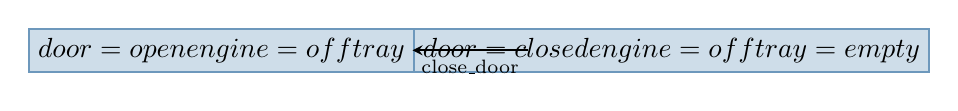
\begin{tikzpicture}[auto]

%
% Styles
%
\tikzstyle{state} = [rectangle,draw=oproverblue!60,fill=oproverblue!20,thick]
\tikzstyle{initialstate} = [rectangle,draw=mydarkgreen!60,fill=mydarkgreen!20,thick]
\tikzstyle{tran}  = [->,>=stealth,semithick]

\node[state] (000) at (  -2.5,  0)  {$\nodd{door=open}{engine=off}{tray=empty}$};
\node[state] (100) at (  2.5,  0)  {$\nodd{door=closed}{engine=off}{tray=empty}$};

\draw[tran] (000) -- node {\scriptsize close\_door} (100);

\end{tikzpicture}
}
  \end{center}
  \pause

  \begin{tabular}{llllcl}
    if & tray=empty  & then & tray'=full & ~~~ & [fill\_tray]
  \end{tabular}

  \begin{center}
  \scalebox{.85}{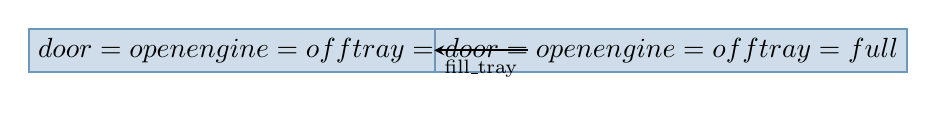
\begin{tikzpicture}[auto]

%
% Styles
%
\tikzstyle{state} = [rectangle,draw=oproverblue!60,fill=oproverblue!20,thick]
\tikzstyle{initialstate} = [rectangle,draw=mydarkgreen!60,fill=mydarkgreen!20,thick]
\tikzstyle{tran}  = [->,>=stealth,semithick]

\node[state] (000) at (  -2.5,  0)  {$\nodd{door=open}{engine=off}{tray=empty}$};
\node[state] (100) at (   2.5,  0)  {$\nodd{door=open}{engine=off}{tray=full}$};

\draw[tran] (000) -- node {\scriptsize fill\_tray} (100);

\end{tikzpicture}
}
  \end{center}
  \pause

  \begin{tabular}{llllcl}
    \multirow{2}{*}{if} & \multirow{2}{*}{door=closed} & \multirow{2}{*}{then} & door'=open  & & \multirow{2}{*}{[open\_door]} \\ 
                        &                              &                       & engine'=off & &                             \\
  \end{tabular}

  \begin{center}
  \scalebox{.85}{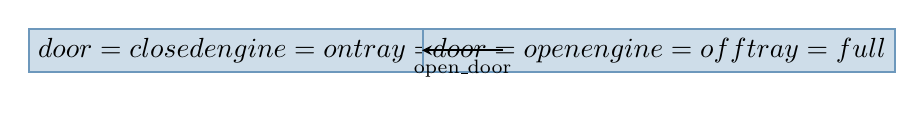
\begin{tikzpicture}[auto]

%
% Styles
%
\tikzstyle{state} = [rectangle,draw=oproverblue!60,fill=oproverblue!20,thick]
\tikzstyle{initialstate} = [rectangle,draw=mydarkgreen!60,fill=mydarkgreen!20,thick]
\tikzstyle{tran}  = [->,>=stealth,semithick]

\node[state] (000) at (  -2.5,  0)  {$\nodd{door=closed}{engine=on}{tray=full}$};
\node[state] (100) at (   2.5,  0)  {$\nodd{door=open}{engine=off}{tray=full}$};

\draw[tran] (000) -- node {\scriptsize open\_door} (100);

\end{tikzpicture}
}
  \end{center}
  \pause

  \begin{tabular}{llllcl}
    \multirow{2}{*}{if} & door=closed & \multirow{2}{*}{then} & tray'=empty & & \multirow{2}{*}{[start\_washing]} \\ 
                        & engine=off  &                       & engine'=on  & &                                   \\
  \end{tabular}

  \begin{center}
  \scalebox{.85}{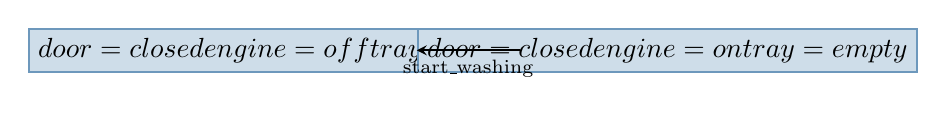
\begin{tikzpicture}[auto]

%
% Styles
%
\tikzstyle{state} = [rectangle,draw=oproverblue!60,fill=oproverblue!20,thick]
\tikzstyle{initialstate} = [rectangle,draw=mydarkgreen!60,fill=mydarkgreen!20,thick]
\tikzstyle{tran}  = [->,>=stealth,semithick]

\node[state] (000) at (  -2.5,  0) {$\nodd{door=closed}{engine=off}{tray=full}$};
\node[state] (100) at (  2.5,  0)  {$\nodd{door=closed}{engine=on}{tray=empty}$};

\draw[tran] (000) -- node {\scriptsize start\_washing} (100);

\end{tikzpicture}
}
  \end{center}

\end{frame}

\begin{frame}
  \frametitle{Modeling - (Safety) Property}

  Last step, we need to model the property
  \begin{center}
    ``when the engine is on the door is closed'' 
  \end{center}
  It is a {\bf safety} property: they are easy
  to define as they are properties of the states
  \vfill\pause
  We call {\bf bad state} (or unsafe state) a state 
  that does not satisfy the property
  \vfill
  \begin{center}
  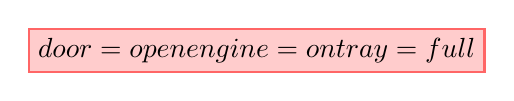
\begin{tikzpicture}[auto]

%
% Styles
%
\tikzstyle{badstate} = [rectangle,draw=red!60,fill=red!20,thick]

\node[badstate] (011) at (  0, 0)  {$\nodd{door=open}{engine=on}{tray=full}$};

\end{tikzpicture}

  \end{center}

\end{frame}

\subsection{Checking}

\begin{frame}
  \frametitle{Checking (= Reachability)}

  To establish if a model satisfies a safety 
  property amounts to check if some
  {\bf bad state is reachable} from the set
  of initial states
  \vfill
  This can be done automatically by {\bf visiting} the
  set of states that are {\bf reachable} from the initial
  state with the application of a transition
  \vfill
  \pause
  Let $S^{(0)}$ be the set of initial states.
  Algorithmically, it amounts to implement the following loop
  (iteration $i$)
  \vfill
  \begin{boxedminipage}{\textwidth}
  \begin{center}
  Forward-Reachability
  \begin{tabular}{rcl}
     \\
       {\bf Safety Check} & ~~ & If $S^{(i)}$ contains a bad state, return {\bf unsafe} \\
        {\bf Next States} & ~~ & Compute $S^{(i+1)} := S^{(i)} \cup T(S^{(i)})$ \\
    {\bf Fix-Point Check} & ~~ & If $S^{(i+1)} \equiv S^{(i)}$, return {\bf safe} 
  \end{tabular}
  \end{center}
  \end{boxedminipage}
  \vfill
  $T(S^{(i)}) = $ states that can be reached from $S^{(i)}$ with a transition

\end{frame}

\begin{frame}
  \frametitle{Checking - Forward Reachability - Property Verified}
  \begin{boxedminipage}{\textwidth}
  \begin{center}
  Forward-Reachability
  \begin{tabular}{rcl}
     \\
       {\bf Safety Check} & ~~ & \colthrat{If $S^{(i)}$ contains a bad state, return {\bf unsafe}}{2,5,8,11|handout:0} \\
        {\bf Next States} & ~~ & \colthrat{Compute $S^{(i+1)} := S^{(i)} \cup T(S^{(i)})$}{3,6,9,12|handout:0} \\
    {\bf Fix-Point Check} & ~~ & \colthrat{If $S^{(i+1)} \equiv S^{(i)}$, return {\bf safe}}{4,7,10,13} 
  \end{tabular}
  \end{center}
  \end{boxedminipage}
  \vfill
  \begin{overlayarea}{\textwidth}{4cm}
    \only<1,2|handout:0>{\scalebox{.6}{\input{forward_1.pdf_t}}}
    \only<3-5|handout:0>{\scalebox{.6}{\input{forward_2.pdf_t}}}
    \only<6-8|handout:0>{\scalebox{.6}{\input{forward_3.pdf_t}}}
    \only<9-11|handout:0>{\scalebox{.6}{\input{forward_4.pdf_t}}}
    \only<12,13>{\scalebox{.6}{\input{forward_5.pdf_t}}}
  \end{overlayarea}

\end{frame}

\begin{frame}
  \frametitle{Checking - Forward Reachability - Property Not Verified}
  \begin{boxedminipage}{\textwidth}
  \begin{center}
  Forward-Reachability
  \begin{tabular}{rcl}
     \\
       {\bf Safety Check} & ~~ & \colthrat{If $S^{(i)}$ contains a bad state, return {\bf unsafe}}{1} \\
        {\bf Next States} & ~~ & Compute $S^{(i+1)} := S^{(i)} \cup T(S^{(i)})$ \\
    {\bf Fix-Point Check} & ~~ & If $S^{(i+1)} \equiv S^{(i)}$, return {\bf safe}
  \end{tabular}
  \end{center}
  \end{boxedminipage}
  \vfill
  \begin{overlayarea}{\textwidth}{4cm}
    \only<1|handout:0>{\scalebox{.6}{\input{forward_6.pdf_t}}}
    \only<2>{\scalebox{.6}{\input{forward_7.pdf_t}}}
  \end{overlayarea}

\end{frame}

\begin{frame}
  \frametitle{Back to the washing machine}

Iteration: \only<1|handout:0>{0}\only<2|handout:0>{1}\only<3|handout:0>{2}\only<4|handout:0>{3}\only<5>{4 - Fix Point Reached - System is SAFE}
  \vfill
  \begin{center}
    \only<1|handout:0>{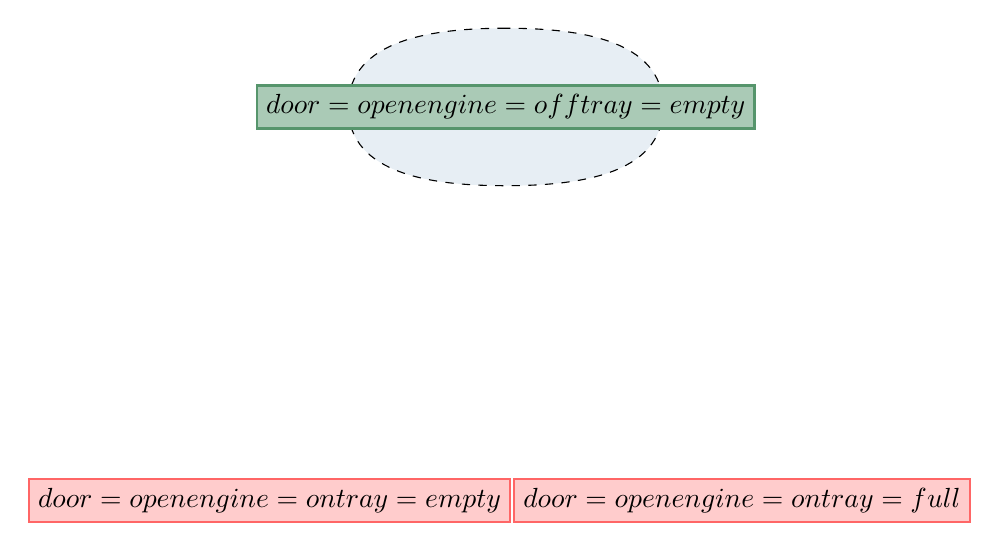
\begin{tikzpicture}[auto]

%
% Styles
%
\tikzstyle{state} = [rectangle,draw=oproverblue!60,fill=oproverblue!20,thick]
\tikzstyle{initialstate} = [rectangle,draw=mydarkgreen!80,fill=mydarkgreen!40,thick]
\tikzstyle{badstate} = [rectangle,draw=red!60,fill=red!20,thick]

\draw[fill=oproverblue!10,dashed] (0, 0) to [out=180,in=90] (-2,-1) 
                                         to [out=-90,in=180]( 0,-2)
                                         to [out=0,in=-90]  ( 2,-1)
                                         to [out=90,in=0]   ( 0, 0);

\node[initialstate] (000) at (  0,  -1)  {$\nodd{door=open}{engine=off}{tray=empty}$};
%\node[state] (100) at ( -4, -2)  {$\nodd{door=closed}{engine=off}{tray=empty}$};
%\node[state] (001) at (  4, -2)  {$\nodd{door=open}{engine=off}{tray=full}$};
%\node[state] (101) at ( -2, -4)  {$\nodd{door=closed}{engine=off}{tray=full}$};
%\node[state] (110) at (  2, -4)  {$\nodd{door=closed}{engine=on}{tray=empty}$};
\node[badstate] (011) at (  3, -6)  {$\nodd{door=open}{engine=on}{tray=full}$};
%\node[state] (111) at ( -3, -6)  {$\nodd{door=closed}{engine=on}{tray=full}$};
\node[badstate] (010) at ( -3, -6)  {$\nodd{door=open}{engine=on}{tray=empty}$};


\end{tikzpicture}
}
    \only<2|handout:0>{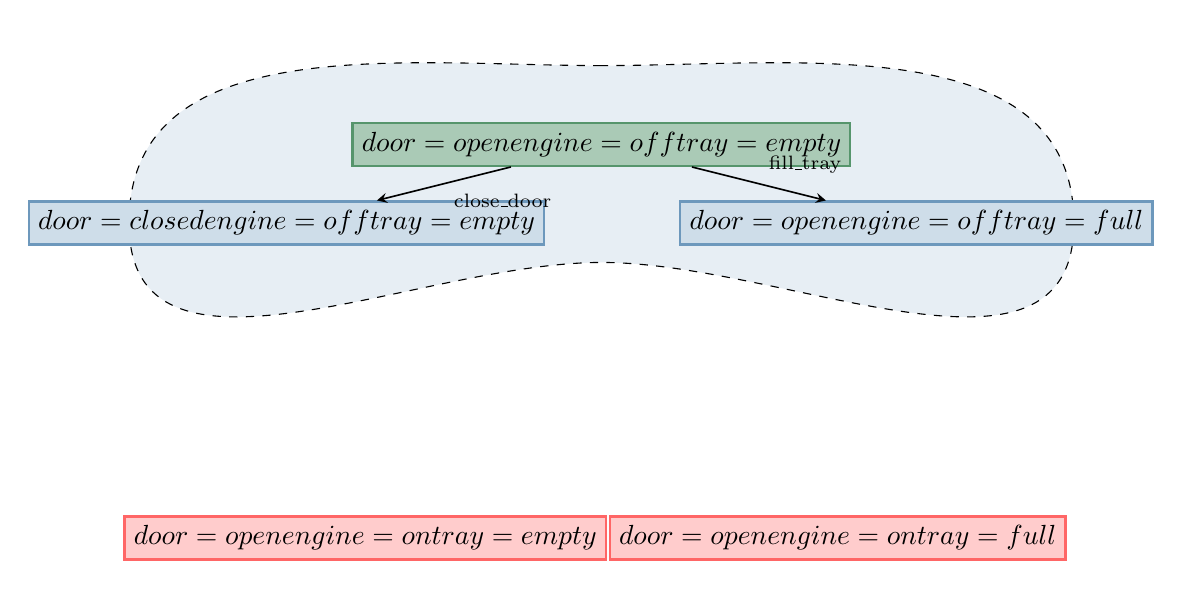
\begin{tikzpicture}[auto]

%
% Styles
%
\tikzstyle{state} = [rectangle,draw=oproverblue!60,fill=oproverblue!20,thick]
\tikzstyle{initialstate} = [rectangle,draw=mydarkgreen!80,fill=mydarkgreen!40,thick]
\tikzstyle{badstate} = [rectangle,draw=red!60,fill=red!20,thick]
\tikzstyle{tran}  = [->,>=stealth,semithick]

\draw[fill=oproverblue!10,dashed] (0, 0) to [out=180,in=90] (-6,-2) 
                                         to [out=-90,in=180]( 0,-2.5)
                                         to [out=0,in=-90]  ( 6,-2)
                                         to [out=90,in=0]   ( 0, 0);

\node[initialstate] (000) at (  0,  -1)  {$\nodd{door=open}{engine=off}{tray=empty}$};
\node[state]        (100) at ( -4,  -2)  {$\nodd{door=closed}{engine=off}{tray=empty}$};
\node[state]        (001) at (  4, -2)   {$\nodd{door=open}{engine=off}{tray=full}$};
%\node[state] (101) at ( -2, -4)  {$\nodd{door=closed}{engine=off}{tray=full}$};
%\node[state] (110) at (  2, -4)  {$\nodd{door=closed}{engine=on}{tray=empty}$};
\node[badstate] (011) at (  3, -6)  {$\nodd{door=open}{engine=on}{tray=full}$};
%\node[state] (111) at ( -3, -6)  {$\nodd{door=closed}{engine=on}{tray=full}$};
\node[badstate] (010) at ( -3, -6)  {$\nodd{door=open}{engine=on}{tray=empty}$};

\draw[tran] (000) -- node {\scriptsize close\_door} (100);
\draw[tran] (000) -- node {\scriptsize fill\_tray}  (001);

\end{tikzpicture}
}
    \only<3|handout:0>{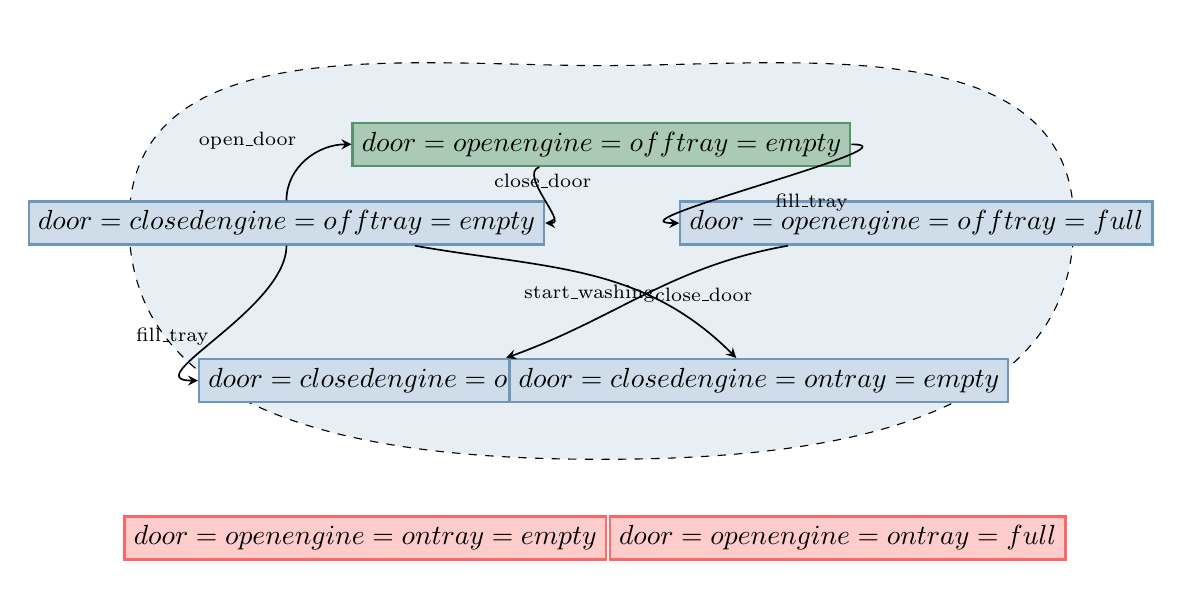
\begin{tikzpicture}[auto]

%
% Styles
%
\tikzstyle{state} = [rectangle,draw=oproverblue!60,fill=oproverblue!20,thick]
\tikzstyle{initialstate} = [rectangle,draw=mydarkgreen!80,fill=mydarkgreen!40,thick]
\tikzstyle{badstate} = [rectangle,draw=red!60,fill=red!20,thick]
\tikzstyle{tran}  = [->,>=stealth,semithick]

\draw[fill=oproverblue!10,dashed] (0, 0) to [out=180,in=90] (-6,-2) 
                                         to [out=-90,in=180]( 0,-5)
                                         to [out=0,in=-90]  ( 6,-2)
                                         to [out=90,in=0]   ( 0, 0);

\node[initialstate] (000) at (  0,  -1)  {$\nodd{door=open}{engine=off}{tray=empty}$};
\node[state]        (100) at ( -4,  -2)  {$\nodd{door=closed}{engine=off}{tray=empty}$};
\node[state]        (001) at (  4, -2)   {$\nodd{door=open}{engine=off}{tray=full}$};
\node[state]        (101) at ( -2, -4)  {$\nodd{door=closed}{engine=off}{tray=full}$};
\node[state]        (110) at (  2, -4)  {$\nodd{door=closed}{engine=on}{tray=empty}$};
\node[badstate]     (011) at (  3, -6)  {$\nodd{door=open}{engine=on}{tray=full}$};
%\node[state] (111) at ( -3, -6)  {$\nodd{door=closed}{engine=on}{tray=full}$};
\node[badstate]     (010) at ( -3, -6)  {$\nodd{door=open}{engine=on}{tray=empty}$};

\draw[tran] (000) to [out=200,in=0]   node[above] {\scriptsize close\_door} (100);
\draw[tran] (000) to [out=0,in=180] node {\scriptsize fill\_tray}  (001);
\draw[tran] (100) to [out=90,in=180]  node {\scriptsize open\_door}  (000);
\draw[tran] (100) to [out=-10,in=135]  node[below] {\scriptsize start\_washing}  (110);
\draw[tran] (100) to [out=-90,in=180]  node[left] {\scriptsize fill\_tray}      (101);
\draw[tran] (001) to [out=190,in=20]   node[right] {\scriptsize close\_door}      (101);

\end{tikzpicture}
}
    \only<4|handout:0>{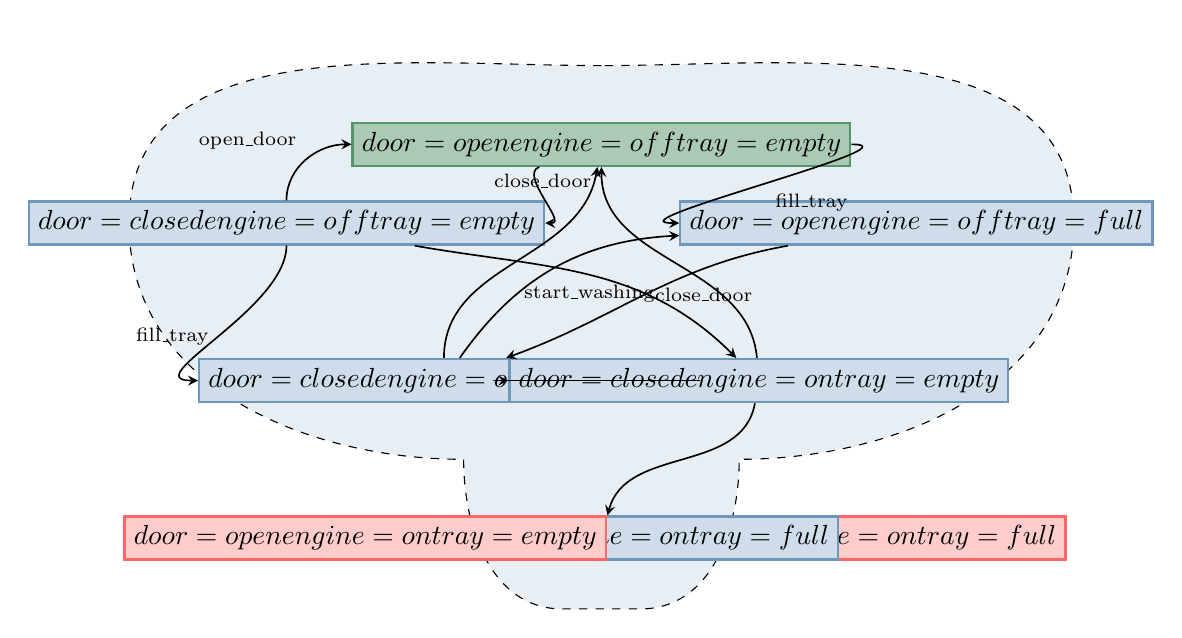
\begin{tikzpicture}[auto]

%
% Styles
%
\tikzstyle{state} = [rectangle,draw=oproverblue!60,fill=oproverblue!20,thick]
\tikzstyle{initialstate} = [rectangle,draw=mydarkgreen!80,fill=mydarkgreen!40,thick]
\tikzstyle{badstate} = [rectangle,draw=red!60,fill=red!20,thick]
\tikzstyle{tran}  = [->,>=stealth,semithick]

\draw[fill=oproverblue!10,dashed] (0, 0) to [out=180,in=90] (-6,-2) 
                                         to [out=-90,in=180]( -1.75,-5)
                                         to [out=-90,in=180] (  -0.5,-6.9)
                                         to [out=0,in=180] (   0.5,-6.9)
                                         to [out=0,in=-90]   (  1.75,-5)
                                         to [out=0,in=-90]  ( 6,-2)
                                         to [out=90,in=0]   ( 0, 0);

\node[initialstate] (000) at (  0,  -1)  {$\nodd{door=open}{engine=off}{tray=empty}$};
\node[state]        (100) at ( -4,  -2)  {$\nodd{door=closed}{engine=off}{tray=empty}$};
\node[state]        (001) at (  4, -2)   {$\nodd{door=open}{engine=off}{tray=full}$};
\node[state]        (101) at ( -2, -4)  {$\nodd{door=closed}{engine=off}{tray=full}$};
\node[state]        (110) at (  2, -4)  {$\nodd{door=closed}{engine=on}{tray=empty}$};
\node[badstate]     (011) at (  3, -6)  {$\nodd{door=open}{engine=on}{tray=full}$};
\node[state]        (111) at (  0, -6)  {$\nodd{door=closed}{engine=on}{tray=full}$};
\node[badstate]     (010) at ( -3, -6)  {$\nodd{door=open}{engine=on}{tray=empty}$};

\draw[tran] (000) to [out=200,in=0]    node[above] {\scriptsize close\_door}    (100);
\draw[tran] (000) to [out=0,in=180]    node {\scriptsize fill\_tray}            (001);
\draw[tran] (100) to [out=90,in=180]   node {\scriptsize open\_door}            (000);
\draw[tran] (100) to [out=-10,in=135]  node[below] {\scriptsize start\_washing} (110);
\draw[tran] (100) to [out=-90,in=180]  node[left] {\scriptsize fill\_tray}      (101);
\draw[tran] (001) to [out=190,in=20]   node[right] {\scriptsize close\_door}    (101);
\draw[tran] (101) to [out=90,in=-100]   (000);
\draw[tran] (101) to [out=55,in=183]    (001);
\draw[tran] (101) to [out=0,in=180]     (110);
\draw[tran] (110) to [out=95,in=-90]    (000);
\draw[tran] (110) to [out=-100,in=75]    (111);
%\draw[tran] (111) to [out=190,in=20]   node[right] {\scriptsize close\_door}    (001);

\end{tikzpicture}
}
    \only<5>{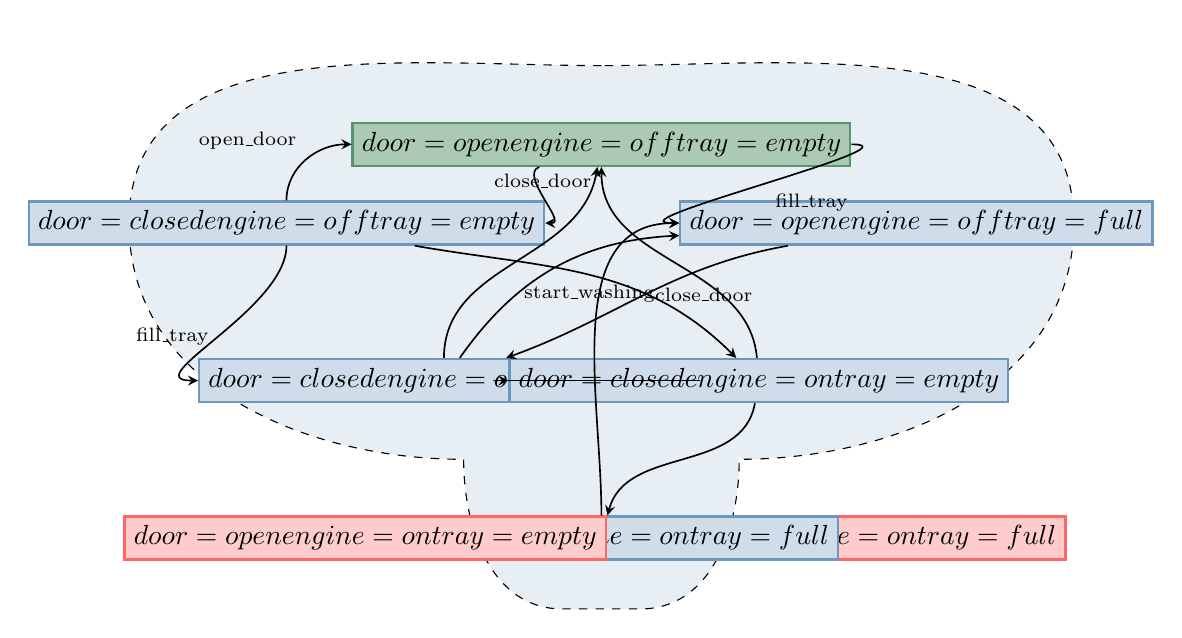
\begin{tikzpicture}[auto]

%
% Styles
%
\tikzstyle{state} = [rectangle,draw=oproverblue!60,fill=oproverblue!20,thick]
\tikzstyle{initialstate} = [rectangle,draw=mydarkgreen!80,fill=mydarkgreen!40,thick]
\tikzstyle{badstate} = [rectangle,draw=red!60,fill=red!20,thick]
\tikzstyle{tran}  = [->,>=stealth,semithick]

\draw[fill=oproverblue!10,dashed] (0, 0) to [out=180,in=90] (-6,-2) 
                                         to [out=-90,in=180]( -1.75,-5)
                                         to [out=-90,in=180] (  -0.5,-6.9)
                                         to [out=0,in=180] (   0.5,-6.9)
                                         to [out=0,in=-90]   (  1.75,-5)
                                         to [out=0,in=-90]  ( 6,-2)
                                         to [out=90,in=0]   ( 0, 0);

\node[initialstate] (000) at (  0,  -1)  {$\nodd{door=open}{engine=off}{tray=empty}$};
\node[state]        (100) at ( -4,  -2)  {$\nodd{door=closed}{engine=off}{tray=empty}$};
\node[state]        (001) at (  4, -2)   {$\nodd{door=open}{engine=off}{tray=full}$};
\node[state]        (101) at ( -2, -4)  {$\nodd{door=closed}{engine=off}{tray=full}$};
\node[state]        (110) at (  2, -4)  {$\nodd{door=closed}{engine=on}{tray=empty}$};
\node[badstate]     (011) at (  3, -6)  {$\nodd{door=open}{engine=on}{tray=full}$};
\node[state]        (111) at (  0, -6)  {$\nodd{door=closed}{engine=on}{tray=full}$};
\node[badstate]     (010) at ( -3, -6)  {$\nodd{door=open}{engine=on}{tray=empty}$};

\draw[tran] (000) to [out=200,in=0]    node[above] {\scriptsize close\_door}    (100);
\draw[tran] (000) to [out=0,in=180]    node {\scriptsize fill\_tray}            (001);
\draw[tran] (100) to [out=90,in=180]   node {\scriptsize open\_door}            (000);
\draw[tran] (100) to [out=-10,in=135]  node[below] {\scriptsize start\_washing} (110);
\draw[tran] (100) to [out=-90,in=180]  node[left] {\scriptsize fill\_tray}      (101);
\draw[tran] (001) to [out=190,in=20]   node[right] {\scriptsize close\_door}    (101);
\draw[tran] (101) to [out=90,in=-100]   (000);
\draw[tran] (101) to [out=55,in=183]    (001);
\draw[tran] (101) to [out=0,in=180]     (110);
\draw[tran] (110) to [out=95,in=-90]    (000);
\draw[tran] (110) to [out=-100,in=75]   (111);
\draw[tran] (111) to [out=90,in=180]    (001);

\end{tikzpicture}
}
  \end{center}

\end{frame}

\begin{frame}
  \frametitle{Checking - Backward Reachability}
  \begin{boxedminipage}{\textwidth}
  \begin{center}
  Backward-Reachability ($S^{(0)} \equiv$ ``bad states'')
  \begin{tabular}{rcl}
     \\
       {\bf Safety Check} & ~~ & If $S^{(i)}$ contains an initial, return {\bf unsafe} \\
        {\bf Next States} & ~~ & Compute $S^{(i+1)} := S^{(i)} \cup T^{-1}(S^{(i)})$ \\
    {\bf Fix-Point Check} & ~~ & If $S^{(i+1)} \equiv S^{(i)}$, return {\bf safe}
  \end{tabular}
  \end{center}
  \end{boxedminipage}
  \vfill
  \begin{overlayarea}{\textwidth}{4cm}
    \only<1|handout:0>{\scalebox{.6}{\input{backward_1.pdf_t}}}
    \only<2>{\scalebox{.6}{\input{backward_2.pdf_t}}}
  \end{overlayarea}

\end{frame}

\subsection{Implementing a Model-Checker}

\begin{frame}
  \frametitle{Implementing a Model-Checker}

  In order to implement model-checker we need: 
  \begin{enumerate}
    \item representing large sets of states
    \item computing $T(S^{(i)})$
    \item check if bad states are in $S^{(i)}$ 
    \item check if $S^{(i)} \equiv S^{(i+1)}$ 
  \end{enumerate}
  \vfill\pause
  The naive way would be to represent states {\bf explicitly} 
  (e.g., with a C {\tt struct} containing values for state variables)
  \vfill
  Very few model-checkers adopt this method (e.g., SPIN)
  \vfill\pause
  A more powerful approach represents 
  states {\bf symbolically}, 
  by means of SAT/SMT-formul\ae: each set of
  states $S$ is represented by a formula $\phi$ such
  that $S$ corresponds to the models of $\phi$

\end{frame}

\begin{frame}
  \frametitle{Symbolic Model-Checking - Representing States}

  \scriptsize

  Examples:
  \medskip\\
  \begin{tabular}{ccc}

    \begin{minipage}{.4\textwidth}
      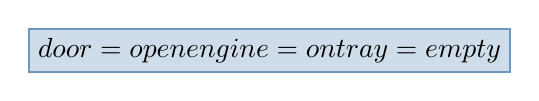
\begin{tikzpicture}[auto]

%
% Styles
%
\tikzstyle{vertex} = [rectangle,draw=oproverblue!60,fill=oproverblue!20,thick]

\node[vertex] (x) at ( 0, 0)  {$\nodd{door=open}{engine=on}{tray=empty}$};

\end{tikzpicture}

    \end{minipage}
    &~ &
    door\_open $\wedge$ engine\_on $\wedge$ $\neg$ tray\_full \\
    \pause
    \\

    \begin{minipage}{.4\textwidth}
      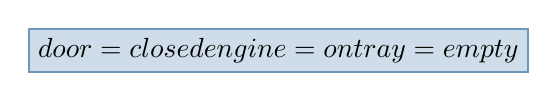
\begin{tikzpicture}[auto]

%
% Styles
%
\tikzstyle{vertex} = [rectangle,draw=oproverblue!60,fill=oproverblue!20,thick]

\node[vertex] (x) at ( 0, 0)  {$\nodd{door=closed}{engine=on}{tray=empty}$};

\end{tikzpicture}

    \end{minipage}
    &~ &
    $\neg$ door\_open $\wedge$ engine\_on $\wedge$ $\neg$ tray\_full \\
    \pause
    \\

    \begin{minipage}{.4\textwidth}
      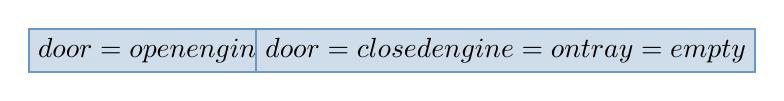
\begin{tikzpicture}[auto]

%
% Styles
%
\tikzstyle{vertex} = [rectangle,draw=oproverblue!60,fill=oproverblue!20,thick]

\node[vertex] (x) at ( 0, 0)  {$\nodd{door=open}{engine=on}{tray=empty}$};
\node[vertex] (y) at ( 3, 0)  {$\nodd{door=closed}{engine=on}{tray=empty}$};

\end{tikzpicture}

    \end{minipage}
    &~ &
    engine\_on $\wedge$ $\neg$ tray\_full \\

  \end{tabular}
  \vfill\pause
  Also, it is easy to see that:
  \medskip\\
  \begin{tabular}{ccc}
    $S_1 \cup S_2$ & & $\phi_1 \vee \phi_2$ \\
    $S_1 \cap S_2$ & & $\phi_1 \wedge \phi_2$ \\
    $S_1 \subseteq S_2$ & & $\phi_1 \rightarrow \phi_2$ 
  \end{tabular}

\end{frame}

\begin{frame}
  \frametitle{Symbolic Model-Checking - Representing Transitions}

  \scriptsize

  Transitions are also represented as formul\ae\xspace between state
  variables and their primed versions 
  \vfill
  \begin{tabular}{llllcl}
    \multirow{2}{*}{if} & door=closed & \multirow{2}{*}{then} & tray'=empty & & \multirow{2}{*}{[start\_washing]} \\ 
                        & engine=off  &                       & engine'=on  & &                                   \\
  \end{tabular}
  \vfill
  $$
    \neg \mbox{door\_open} \wedge \neg \mbox{engine\_on} \wedge \neg \mbox{door\_open'} \wedge \mbox{engine\_on'} \wedge \neg \mbox{tray\_full'}
  $$
  \vfill\pause
  This formula says that the following pair of states are related
  $$
  \begin{array}{rcl}
    \neg \mbox{door\_open} \wedge \neg \mbox{engine\_on} \wedge \neg \mbox{tray\_full} 
    & ~~~ & \neg \mbox{door\_open'} \wedge \mbox{engine\_on'} \wedge \neg \mbox{tray\_full'} \\
    \\
    \neg \mbox{door\_open} \wedge \neg \mbox{engine\_on} \wedge \mbox{tray\_full} 
    & ~~~ & \neg \mbox{door\_open'} \wedge \mbox{engine\_on'} \wedge \neg \mbox{tray\_full'} 
  \end{array}
  $$

\end{frame}

\begin{frame}
  \frametitle{Symbolic Model-Checking - Computing Next State}

  \scriptsize

  From a set of states $S^{(i)}$, represented symbolically by a formula $\phi( \vec{s} )$,
  and a transition $t_j$, represented symbolically by a formula $\psi( \vec{s}, \vec{s'} )$,
  the next states $t_j(S^{(i)})$ can be expressed as
  $$
  \exists \vec{s}.\ \phi( \vec{s} ) \wedge \psi( \vec{s}, \vec{s'} )
  $$
  By means of an operation called {\bf quantifier elimination}, we can remove $\vec{s}$.
  If then we rename $\vec{s'}$ as $\vec{s}$ we obtain the symbolic representation of $t_j(S^{(i)})$
  \vfill\pause
  Example:
  $$
  \begin{array}{l}
    \phi \equiv \neg \mbox{door\_open} \wedge \neg \mbox{engine\_on} \\
    \psi \equiv \neg \mbox{door\_open} \wedge \neg \mbox{engine\_on} \wedge 
                \neg \mbox{door\_open'} \wedge \mbox{engine\_on'} \wedge \neg \mbox{tray\_full'} \\
  \end{array}
  $$
  Quantifier elimination of $\exists \mbox{ door\_open}, \mbox{engine\_on}.\ \phi \wedge \psi$ is
  $$
    \neg \mbox{door\_open'} \wedge \mbox{engine\_on'} \wedge \neg \mbox{tray\_full'} 
  $$
  and therefore
  $$
    \neg \mbox{door\_open} \wedge \mbox{engine\_on} \wedge \neg \mbox{tray\_full} 
  $$
  is $t_j(S^{(i)})$. The whole set of next states $T(S^{(i)})$ is 
  $\bigvee_j t_j( S^{(i)} )$

\end{frame}

\begin{frame}
  \frametitle{Symbolic Model-Checking - Bad states in $S^{(i)}$}

  Suppose that $\phi$ is the symbolic representation of $S^{(i)}$,
  and that $\beta$ is the symbolic representation of the {\bf bad states}
  \vfill
  checking if some bad state is in $S^{(i)}$ can be simply done with\pause
  $$
    \phi \wedge \beta \mbox{ is satisfiable ?}
  $$

\end{frame}

\begin{frame}
  \frametitle{Symbolic Model-Checking - Fix point test}

  Suppose that $\phi_i$ is the symbolic representation of $S^{(i)}$
  and that $\phi_{i+1}$ is the symbolic representation of $S^{(i+1)}$
  how do I that $S^{(i)} \equiv S^{(i+1)}$ ?
  \vfill\pause
  First of all, notice that $S^{(i)} \equiv S^{(i+1)}$ if and only if
  $$
    S^{(i)} \subseteq S^{(i+1)} \mbox{ and } S^{(i+1)} \subseteq S^{(i)}
  $$
  \vfill\pause
  $S^{(i)} \subseteq S^{(i+1)}$ always holds (explored states grow monotonically)
  \vfill\pause
  $S^{(i+1)} \subseteq S^{(i)}$ can be perfomed with the following check
  $$
  \begin{array}{l}
    \phi_{i+1} \rightarrow \phi_i \mbox{ is a tautology ? or equivalently} \\
    \phi_{i+1} \wedge \neg \phi_i \mbox{ is unsafisfiable ? } 
  \end{array}
  $$

\end{frame}

\begin{frame}
  \frametitle{Symbolic Model-Checking - Summary}

  Model-Checking can be implemented by representing
  states and transitions symbolically with SAT/SMT-formul\ae
  \vfill
  Next states $T(S^{(i)})$ can be computed using quantifier elimination
  \vfill
  Presence of bad states can be computed with a satisfiability call of
  the form $\phi \wedge \beta$
  \vfill
  Fix-point check can be computed with a satisfiability call of the
  form $\phi_{i+1} \wedge \neg \phi_i$

\end{frame}

\begin{frame}
  \frametitle{Symbolic Model-Checking - Termination}

  \begin{boxedminipage}{\textwidth}
  \begin{center}
  Forward-Reachability
  \begin{tabular}{rcl}
     \\
       {\bf Safety Check} & ~~ & If $\phi_i \wedge \beta$ is satisfiable, return {\bf unsafe} \\
        {\bf Next States} & ~~ & Compute $\phi_{i+1}$ with quantifier elimination \\
    {\bf Fix-Point Check} & ~~ & If $\phi_{i+1} \wedge \neg \phi_i$ is unsatisfiable, return {\bf safe} 
  \end{tabular}
  \end{center}
  \end{boxedminipage}
  \vfill
  Model-Checking always terminates if the satisfiability
  tests above terminates
  \begin{itemize}

    \item If the system under inspection 
	  is a {\bf finite state machine}, everything can be encoded
	  into Booleans, and so they always terminate (SAT-solver is enough)

    \item If the system has {\bf infinite states} (e.g., $0 \leq x \wedge y \geq 2$), 
	  it terminates if everyting can be encoded into a decidable SMT theory
	  (e.g., \Lia) (SMT-Solver necessary)

    \item If quantifiers are needed to express states, then Forward-Reachability
          might not terminate (SMT-Solver plus clever way of handling quantifiers)

  \end{itemize}

\end{frame}


\begin{frame}
  \frametitle{Outline}
  \tableofcontents
\end{frame}

\section{\mcmt}
\begin{frame}
  \frametitle{\mcmt: Model-Checking Modulo Theories}

  \mcmt is a Model-Checker invented and developed by S. Ghilardi and S. Ranise et al.
  (see http://www.dsi.unimi.it/~ghilardi/mcmt/ for complete and precise 
   acknowledgements) 
  \vfill
  It implements a Symbolic Backward-Reachability algorithm (it relies on yices)
  \vfill
  It was invented to handle safety properties for 
  distributed algorithms (protocols), which
  are infinite-state systems
   
\end{frame}

\subsection{Two simple protocols}

\begin{frame}
  \frametitle{\mcmt demo}
  The following example is taken from the tutorial 
  \vfill
  \begin{center}
  Model Checking Modulo Theories: Theory and Practice
  \end{center}
  \vfill
  available at \url{http://st.fbk.eu/MCMTtutorial}
\end{frame}

\begin{frame}
  \frametitle{A simple protocol}
  \framesubtitle{Description}

  \begin{columns}
  \begin{column}{0.3\textwidth}
    \centering
    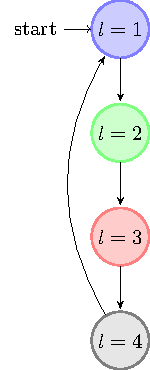
\includegraphics{pictures/demo-prot1-fig}
  \end{column}

  \begin{column}{0.7\textwidth}
    \begin{itemize}
      \item No data, only locations

      \item All processes start from the $1^{\text{st}}$ location

      \item A process in location $3$ is inside the critical section

      \item We want to check if the protocol ensures the mutual exclusion,
	    i.e., at most one process is inside the critical section

    \end{itemize}
  \end{column}

  \end{columns}  

\end{frame}

\begin{frame}[fragile]
  \frametitle{A simple protocol}
  \framesubtitle{Variable}

\begin{columns}
\begin{column}{0.3\textwidth}
\centering
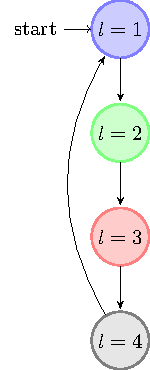
\includegraphics{pictures/demo-prot1-fig}
\end{column}

\begin{column}{0.7\textwidth}
  \begin{itemize}
    \item One {\it local} variable {\tt l}
  \end{itemize}
{\small  
  \begin{verbatim}
  :smt (define-type locations (subrange 1 4))

  :local l locations
  \end{verbatim}
}
\end{column}

\end{columns}  

\end{frame}

\begin{frame}[fragile]
  \frametitle{A simple protocol}
  \framesubtitle{Initial configuration}

  \begin{columns}
  \begin{column}{0.3\textwidth}
  \centering
  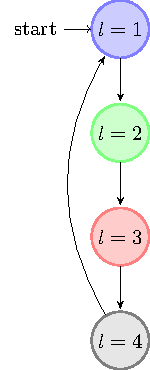
\includegraphics{pictures/demo-prot1-fig}
  \end{column}
  \begin{column}{0.7\textwidth}
  
  \begin{itemize}
    \item All processes start in location $1$
  \end{itemize}

  $$
  \forall x. ({\tt l}[x] = 1)
  $$

  \pause

  \begin{verbatim}
  :initial
  :var x
  :cnj (= l[x] 1)
  \end{verbatim}
  \end{column}

  \end{columns}  

\end{frame}

\begin{frame}[fragile]
  \frametitle{A simple protocol}
  \framesubtitle{Unsafe configuration}

  \begin{columns}
  \begin{column}{0.3\textwidth}
  \centering
  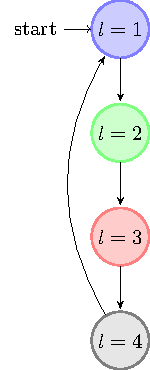
\includegraphics{pictures/demo-prot1-fig}
  \end{column}
  \begin{column}{0.7\textwidth}
  
  \begin{itemize}
    \item Mutual exclusion: At most one process is in location $3$
  \end{itemize}

\pause

\only<1|handout:0>{
$$
U:=\neg\forall z_1, z_2. \left( \left( {\tt l}[z_1] = 3 \wedge {\tt l}[z_2] = 3 \right) \Rightarrow z_1 = z_2 \right)
$$
}
\only<2->{
$$
U:=\exists z_1, z_2. \left( {\tt l}[z_1] = 3 \wedge  {\tt l}[z_2] = 3 \wedge z_1 \neq z_2 \right)
$$
}

\pause
  
  \begin{verbatim}
  :unsafe
  :var z1
  :var z2
  :cnj (= l[z1] 3) (= l[z2] 3)
  \end{verbatim}
\end{column}

\end{columns}  

\end{frame}

\begin{frame}[fragile]
  \frametitle{A simple protocol}
  \framesubtitle{Transitions}

  \begin{columns}
  \begin{column}{0.3\textwidth}
  \centering
  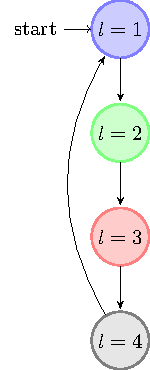
\includegraphics{pictures/demo-prot1-fig}
  \end{column}
  \begin{column}{0.7\textwidth}
  
  \begin{itemize}
    \item A process in location $1$ moves to location $2$
  \end{itemize}

  \vspace{-0.5cm}

  $$
  \tau_1:= \exists x. \left(
  \begin{aligned}
  & {\tt l}[x] = 1 ~\wedge\\
  & {\tt l}' = \lambda j. \left({\sf if}~(x = j)~{\sf then}~2~{\sf else}~{\tt l}[j]\right)
  \end{aligned}
  \right)
  $$
  \pause
 {\footnotesize 
  \begin{verbatim}
  :transition
  :var x
  :var j
  :guard (= l[x] 1)
  :numcases 2
  :case (= x j)
   :val 2
  :case (not (= x j))
   :val l[j]
  \end{verbatim}
 }
\end{column}

\end{columns}  

\end{frame}

\begin{frame}[fragile]
  \frametitle{A simple protocol}
  \framesubtitle{Transitions}

  \begin{columns}
  \begin{column}{0.3\textwidth}
  \centering
  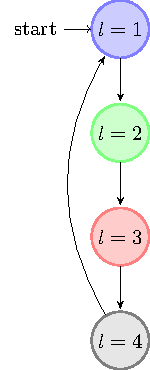
\includegraphics{pictures/demo-prot1-fig}
  \end{column}
  \begin{column}{0.7\textwidth}
  
\begin{columns}
\begin{column}{0.35\textwidth}
 {\scriptsize 
  \begin{verbatim}
  :transition
  :var x
  :var j
  :guard (= l[x] 1)
  :numcases 2
  :case (= x j)
   :val 2
  :case (not (= x j))
   :val l[j]

  :transition
  :var x
  :var j
  :guard (= l[x] 3)
  :numcases 2
  :case (= x j)
   :val 4
  :case (not (= x j))
   :val l[j]
 \end{verbatim}
 }
\end{column}
\begin{column}{0.35\textwidth}
 {\scriptsize 
  \begin{verbatim}
  :transition
  :var x
  :var j
  :guard (= l[x] 2)
  :numcases 2
  :case (= x j)
   :val 3
  :case (not (= x j))
   :val l[j]
  
  :transition
  :var x
  :var j
  :guard (= l[x] 4)
  :numcases 2
  :case (= x j)
   :val 1
  :case (not (= x j))
   :val l[j]
 \end{verbatim}
 }
\end{column}

\end{columns}  

\end{column}

\end{columns}

\end{frame}

\begin{frame}[fragile]
  \frametitle{A simple protocol}
  \framesubtitle{Execution}

  \begin{columns}
  \begin{column}{0.3\textwidth}
  \centering
  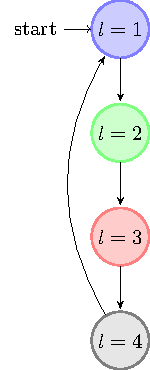
\includegraphics{pictures/demo-prot1-fig}
  \end{column}
  \begin{column}{0.7\textwidth}
  
  \begin{itemize}
    \item {\tt \$ ./mcmt simple\_unsafe.in}
  \end{itemize}

\end{column}

\end{columns}  

\end{frame}




\begin{frame}[fragile]
  \frametitle{A simple protocol}
  \framesubtitle{Execution - Get informations from counterexample}

{\scriptsize
\begin{verbatim}
[...]
Doing state space exploration...
 node 1= [t2_1][0]  
 node 2= [t1_1][t2_1][0]  
 node 3= [t2_2][t2_1][0]  
 node 4= [t2_2][t1_1][t2_1][0]  
 node 5= [t4_1][t1_1][t2_1][0]  
 node 6= [t1_2][t2_2][t1_1][t2_1][0]

=============================================================================
System is UNSAFE!
[...]
\end{verbatim}
}

\end{frame}




\begin{frame}[fragile]
  \frametitle{A simple protocol}
  \framesubtitle{Counterexample analysis from trace}

\begin{tabular}{rl}
Initial state: & $\forall i.\ (\ {\tt l}[i] = 1\ )$ \\
 Unsafe state: & $\exists {\tt z1}, {\tt z2}.\ (\ {\tt l[z1]}=3 \wedge {\tt l[z2]}=3\ )$ \\
 Counter-example: & \verb|node 6 = |\color<9,10>{red}{\verb|[t1_2]|}\color<7,8>{red}{\verb|[t2_2]|}\color<5,6>{red}{\verb|[t1_1]|}\color<3,4>{red}{\verb|[t2_1]|}\color<2>{red}{\verb|[0]|} 
\end{tabular}

\vfill

\only<1,2|handout:0>{ 
\textcolor{white}{
$$
\tau_2:= \exists x. \left(
\begin{aligned}
& {\tt l}[x] = 2 ~\wedge\\
& {\tt l}' = \lambda j. \left({\sf if}~(x = j)~{\sf then}~3~{\sf else}~{\tt l}[j]\right)
\end{aligned}
\right)
$$
}}
\only<3-4,7-8|handout:0>{ 
$$
\tau_2:= \exists x. \left(
\begin{aligned}
& {\tt l}[x] = 2 ~\wedge\\
& {\tt l}' = \lambda j. \left({\sf if}~(x = j)~{\sf then}~3~{\sf else}~{\tt l}[j]\right)
\end{aligned}
\right)
$$
}
\only<5-6,9-10>{ 
$$
\tau_1:= \exists x. \left(
\begin{aligned}
& {\tt l}[x] = 1 ~\wedge\\
& {\tt l}' = \lambda j. \left({\sf if}~(x = j)~{\sf then}~2~{\sf else}~{\tt l}[j]\right)
\end{aligned}
\right)
$$
}

\vfill

\pause

\begin{tabular}{r|l}

\begin{minipage}{.3\textwidth}
\begin{overlayarea}{\textwidth}{3cm}
\only<2,3|handout:0>{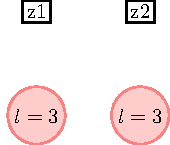
\includegraphics{pictures/demo-prot1-cex-1-fig}}
\only<4,5|handout:0>{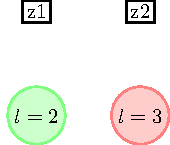
\includegraphics{pictures/demo-prot1-cex-2-fig}}
\only<6,7|handout:0>{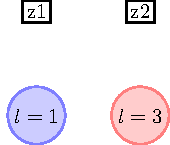
\includegraphics{pictures/demo-prot1-cex-3-fig}}
\only<8,9|handout:0>{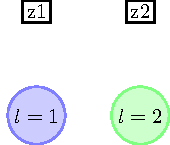
\includegraphics{pictures/demo-prot1-cex-4-fig}}
\only<10>{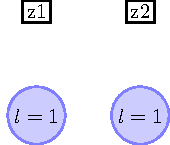
\includegraphics{pictures/demo-prot1-cex-5-fig}}
\end{overlayarea}
\end{minipage}

&

\begin{minipage}{.7\textwidth}
\begin{tabular}{rcl}
     \verb|[0]| & & $\exists {\tt z1}, {\tt z2}.\ (\ {\tt l[z1]}=3 \wedge {\tt l[z2]}=3\ )$ \\
 \pause
 \pause
 \verb|[t2_1]| & & $\exists {\tt z1}, {\tt z2}.\ (\ {\tt l[z1]}=2 \wedge {\tt l[z2]}=3\ )$ \\
 \pause
 \pause
 \verb|[t1_1]| & & $\exists {\tt z1}, {\tt z2}.\ (\ {\tt l[z1]}=1 \wedge {\tt l[z2]}=3\ )$ \\
 \pause
 \pause
 \verb|[t2_2]| & & $\exists {\tt z1}, {\tt z2}.\ (\ {\tt l[z1]}=1 \wedge {\tt l[z2]}=2\ )$ \\
 \pause
 \pause
 \verb|[t1_2]| & & $\exists {\tt z1}, {\tt z2}.\ (\ {\tt l[z1]}=1 \wedge {\tt l[z2]}=1\ )$
\end{tabular}
\end{minipage}

\end{tabular}

\end{frame}




\begin{frame}
  \frametitle{Another simple protocol}
  \framesubtitle{Description}

\begin{columns}
\begin{column}{0.3\textwidth}
\centering
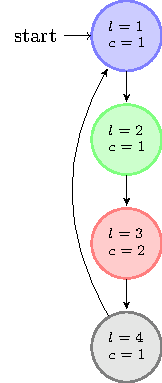
\includegraphics{pictures/demo-prot2-fig}
\end{column}


\begin{column}{0.7\textwidth}
  \begin{itemize}
    \item Like before, but with a \hl{global} flag {\tt c} that
          takes care of mutual exclusion

    \item All processes start from the $1^{\text{st}}$ location

    \item A process in location $3$ is inside the critical section

    \item We want to check if the protocol ensures the mutual exclusion,
	  i.e., at most one process is inside the critical section
  \end{itemize}
\end{column}

\end{columns}  

\end{frame}




\begin{frame}[fragile]
  \frametitle{Another simple protocol}
  \framesubtitle{Variable(s)}

\begin{columns}
\begin{column}{0.3\textwidth}
\centering
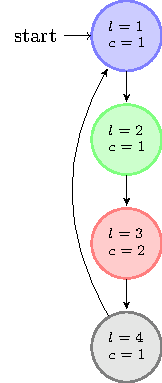
\includegraphics{pictures/demo-prot2-fig}
\end{column}


\begin{column}{0.7\textwidth}
  \begin{itemize}
    \item One {\it local} variable {\tt l}
  \end{itemize}
{\small  
  \begin{verbatim}
  :smt (define-type locations (subrange 1 4))
  :smt (define-type counter (subrange 1 2))

  :local l location
  :global c counter
  \end{verbatim}
}
\end{column}

\end{columns}  

\end{frame}




\begin{frame}[fragile]
  \frametitle{Another simple protocol}
  \framesubtitle{Initial configuration}

\begin{columns}
\begin{column}{0.3\textwidth}
\centering
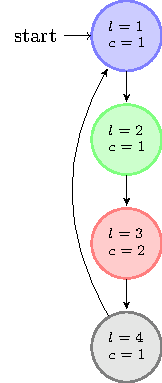
\includegraphics{pictures/demo-prot2-fig}
\end{column}
\begin{column}{0.7\textwidth}
  
  \begin{itemize}
    \item All processes start in location $1$, with counter set to $1$
  \end{itemize}

$$
\forall x.\ (\ {\tt l}[x] = 1 \wedge {\tt c}[x] = 1\ ) 
$$

\pause

  \begin{verbatim}
  :initial
  :var x
  :cnj (= l[x] 1) (= c[x] 1)
  \end{verbatim}
\end{column}

\end{columns}  

\end{frame}



\begin{frame}[fragile]
  \frametitle{Another simple protocol}
  \framesubtitle{Unsafe configuration}

\begin{columns}
\begin{column}{0.3\textwidth}
\centering
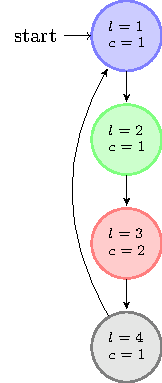
\includegraphics{pictures/demo-prot2-fig}
\end{column}
\begin{column}{0.7\textwidth}
  
  \begin{itemize}
    \item Mutual exclusion: At most one process is in location $3$
  \end{itemize}

\pause

\only<1|handout:0>{
$$
U:=\neg\forall z_1, z_2. \left( \left( {\tt l}[z_1] = 3 \wedge {\tt l}[z_2] = 3 \right) \Rightarrow z_1 = z_2 \right)
$$
}
\only<2->{
$$
U:=\exists z_1, z_2. \left( {\tt l}[z_1] = 3 \wedge  {\tt l}[z_2] = 3 \wedge z_1 \neq z_2 \right)
$$
}

\pause
  
  \begin{verbatim}
  :unsafe
  :var z1
  :var z2
  :cnj (= l[z1] 3) (= l[z2] 3)
  \end{verbatim}
\end{column}

\end{columns}  

\end{frame}





\begin{frame}[fragile]
  \frametitle{Another simple protocol}
  \framesubtitle{Transitions}

\begin{columns}
\begin{column}{0.3\textwidth}
\centering
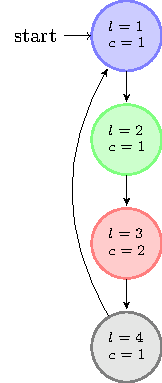
\includegraphics{pictures/demo-prot2-fig}
\end{column}
\begin{column}{0.7\textwidth}
  
%  \begin{itemize}
%    \item A process in location $2$, can move to location $3$ only if $c = 1$.
%  \end{itemize}

%\vspace{-0.5cm}

{\footnotesize
$$
\tau_2:= \exists x. \left(
\begin{aligned}
& {\tt l}[x] = 2 \wedge {\tt c}[x] = 1\ \wedge \\
& {\tt l}' = \lambda j. \left({\sf if}~(x = j)~{\sf then}~3~{\sf else}~{\tt l}[j]\right) \\
& {\tt c}' = \lambda j. 2
\end{aligned}
\right)
$$
}

\vspace{-14pt}

\pause
 {\footnotesize 
  \begin{verbatim}
  :transition
  :var x
  :var j
  :guard (= l[x] 2) (= c[x] 1)
  :numcases 2
  :case (= x j)
   :val 3
   :val 2
  :case (not (= x j))
   :val l[j]
   :val 2
  \end{verbatim}
 }
\end{column}

\end{columns}  

\end{frame}





\begin{frame}[fragile]
  \frametitle{Another simple protocol}
  \framesubtitle{Transitions}

\begin{columns}
\begin{column}{0.3\textwidth}
\centering
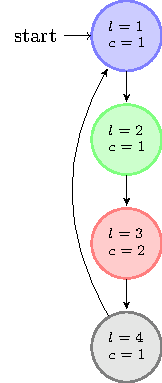
\includegraphics{pictures/demo-prot2-fig}
\end{column}
\begin{column}{0.7\textwidth}
  
\begin{columns}
\begin{column}{0.35\textwidth}
 {\tiny 
  \begin{verbatim}
  :transition
  :var x
  :var j
  :guard (= l[x] 1) 
  :numcases 2
  :case (= x j)
   :val 2
   :val c[x]
  :case (not (= x j))
   :val l[j]
   :val c[x]

  :transition
  :var x
  :var j
  :guard (= l[x] 3) (= c[x] 2)
  :numcases 2
  :case (= x j)
   :val 4
   :val 1
  :case (not (= x j))
   :val l[j]
   :val 1
 \end{verbatim}
 }
\end{column}
\begin{column}{0.35\textwidth}
 {\tiny 
  \begin{verbatim}
  :transition
  :var x
  :var j
  :guard (= l[x] 2) (= c[x] 1)
  :numcases 2
  :case (= x j)
   :val 3
   :val 2
  :case (not (= x j))
   :val l[j]
   :val 2
  
  :transition
  :var x
  :var j
  :guard (= l[x] 4) 
  :numcases 2
  :case (= x j)
   :val 1
   :val c[j]
  :case (not (= x j))
   :val l[j]
   :val c[j]
 \end{verbatim}
 }
\end{column}

\end{columns}  

\end{column}

\end{columns}

\end{frame}






\begin{frame}[fragile]
  \frametitle{Another simple protocol}
  \framesubtitle{Execution}

\begin{columns}
\begin{column}{0.3\textwidth}
\centering
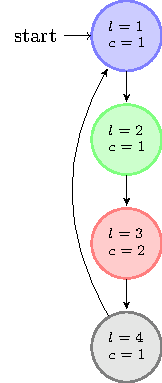
\includegraphics{pictures/demo-prot2-fig}
\end{column}
\begin{column}{0.7\textwidth}
  
  \begin{itemize}
    \item {\tt \$ ./mcmt simple\_safe.in}
  \end{itemize}

\end{column}

\end{columns}  

\end{frame}




\begin{frame}[fragile]
  \frametitle{Another simple protocol}
  \framesubtitle{Execution}

{\scriptsize
\begin{verbatim}
[...]
Doing state space exploration...
 node 1 = [t2_1][0]  
 node 2 = [t1_1][t2_1][0]  
 node 3 = [t4_1][t1_1][t2_1][0]  

=============================================================================
Global fixpoint reached!

System is SAFE!
[...]
\end{verbatim}
}

\end{frame}




\begin{frame}[fragile]
  \frametitle{A simple protocol}
  \framesubtitle{Set of (un)reachable states}

\begin{tabular}{rl}
Initial state: & $\forall i.\ (\ {\tt l}[i] = 1 \wedge {\tt c}[i] = 1\ )$ \\
 Unsafe state: & $\exists {\tt z1}, {\tt z2}.\ (\ {\tt l[z1]}=3 \wedge {\tt l[z2]}=3\ )$ \\
\end{tabular}

\vfill

\begin{columns}

\begin{column}{.3\textwidth}
\begin{overlayarea}{\textwidth}{7cm}
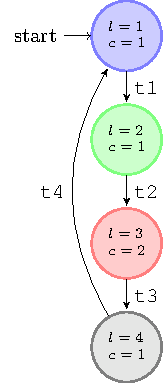
\includegraphics[scale=.8]{pictures/demo-prot2-s-fig}
\end{overlayarea}
\end{column}

\begin{column}{.18\textwidth}
\begin{overlayarea}{\textwidth}{8cm}
\only<1|handout:0>{\vspace{150pt}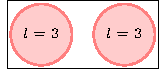
\includegraphics[scale=.6]{pictures/demo-prot2-s-1-fig}}
\only<2|handout:0>{\vspace{113pt}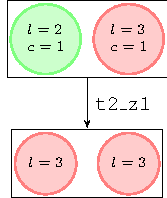
\includegraphics[scale=.6]{pictures/demo-prot2-s-2-fig}}
\only<3|handout:0>{\vspace{77pt}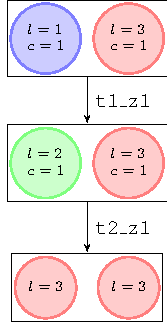
\includegraphics[scale=.6]{pictures/demo-prot2-s-3-fig}}
\only<4|handout:0>{\vspace{41pt}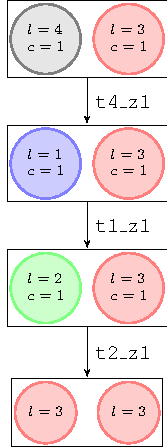
\includegraphics[scale=.6]{pictures/demo-prot2-s-4-fig}}
\only<5|handout:0>{\vspace{5pt}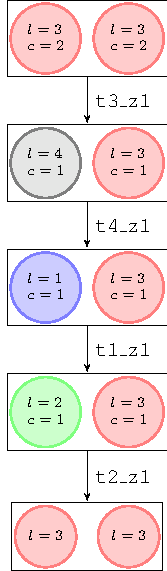
\includegraphics[scale=.6]{pictures/demo-prot2-s-5-fig}}
\only<6>{\vspace{41pt}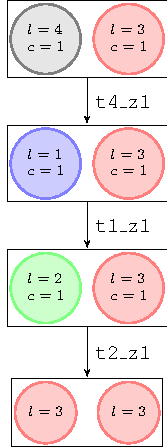
\includegraphics[scale=.6]{pictures/demo-prot2-s-4-fig}}
\end{overlayarea}
\end{column}

\begin{column}{.52\textwidth}
\vspace{-1cm}
{\scriptsize
$$
\tau_1 := \exists x. \left(
\begin{aligned}
& {\tt l}[x] = 1 \ \wedge \\
& {\tt l}' = \lambda j. \left({\sf if}~(x = j)~{\sf then}~2~{\sf else}~{\tt l}[j]\right) \\
& {\tt c}' = \lambda j. {\tt c}[j]
\end{aligned}
\right)
$$
$$
\tau_2 := \exists x. \left(
\begin{aligned}
& {\tt l}[x] = 2 \wedge {\tt c}[x] = 1\ \wedge \\
& {\tt l}' = \lambda j. \left({\sf if}~(x = j)~{\sf then}~3~{\sf else}~{\tt l}[j]\right) \\
& {\tt c}' = \lambda j. 2
\end{aligned}
\right)
$$
$$
\tau_3 := \exists x. \left(
\begin{aligned}
& {\tt l}[x] = 3 \wedge {\tt c}[x] = 2\ \wedge \\
& {\tt l}' = \lambda j. \left({\sf if}~(x = j)~{\sf then}~4~{\sf else}~{\tt l}[j]\right) \\
& {\tt c}' = \lambda j. 1
\end{aligned}
\right)
$$
$$
\tau_4 := \exists x. \left(
\begin{aligned}
& {\tt l}[x] = 4 \ \wedge \\
& {\tt l}' = \lambda j. \left({\sf if}~(x = j)~{\sf then}~1~{\sf else}~{\tt l}[j]\right) \\
& {\tt c}' = \lambda j. {\tt c}[j]
\end{aligned}
\right)
$$
}
\end{column}

\end{columns}

\end{frame}


\end{document}
